\section{Introduction}
\label{sec:Introduction}

\subsection{Background}
\label{sec:Introduction>Background}
Generating content for computer games, CGI effects, feature films, print media, or Role-playing games is a significant bottleneck in terms of effort and resources. A typical game contains many thousands of audio files, images, textures, and 3D models. Procedurally generated content provides a cost-effective alternative to the manual creation of models, textures, images, and sound assets and can expand playability beyond what is otherwise possible. The video game ``No Man's Sky,'' for example, was released in 2016 and relied on procedural asset generation to create over 18 quintillion planets each of which has a unique ecosystem composed of flora and fauna. Such a scale is, of course, beyond the reach of any manually created system. Figure \ref{fig:Screenshot NoManSky} is a screenshot of a planetary terrain region of ``No Man's Sky.''

\begin{figure}[!htb]
\centering
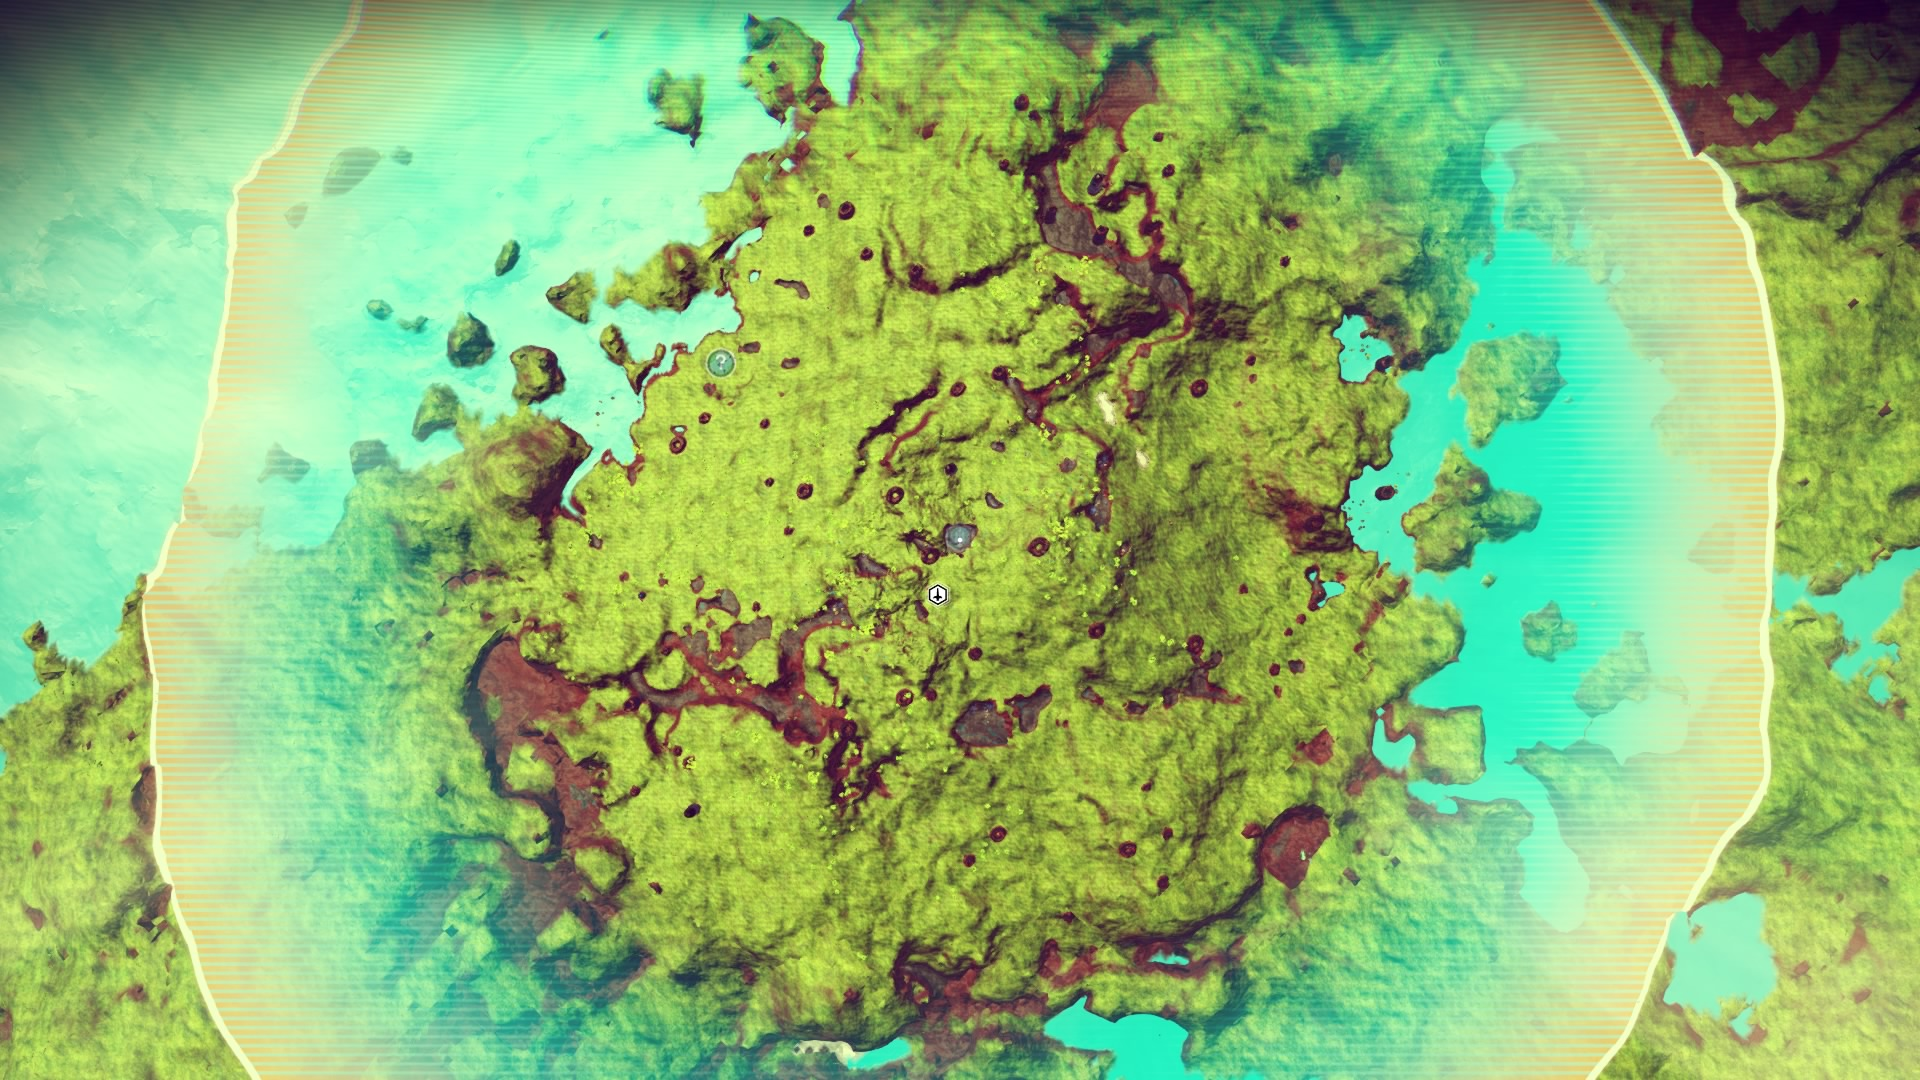
\includegraphics[width=\textwidth]{section01/assets/screenshot_NoManSky.jpg}
\caption[A screenshot of a planetary terrain region of ``No Man's Sky'']{\label{fig:Screenshot NoManSky}A screenshot of a planetary terrain region of ``No Man's Sky''}
\end{figure}

\subsection{Similar Systems}
\label{sec:Introduction>Similar Systems}
% The goal of this project is to automatically generate city maps for use in Role-playing games or world building narratives.
\subsubsection{Minecraft}
\label{sec:Introduction>Similar Systems>Minecraft}
``Minecraft'' is a computer game that can produce massive worlds composed of fine details, like elaborate cliff faces and waterfalls. Moreover, it relies on procedural generation, which automatically creates environments and objects that are at once random but guided by rules that maintain a consistent logic. Mountains are always rocky and sprinkled with snow, for example, while the low lands are typically full of grass and trees. Figure \ref{fig:Screenshot Minecraft} is a screenshot of ``Minecraft.''

\begin{figure}[!htb]
\centering
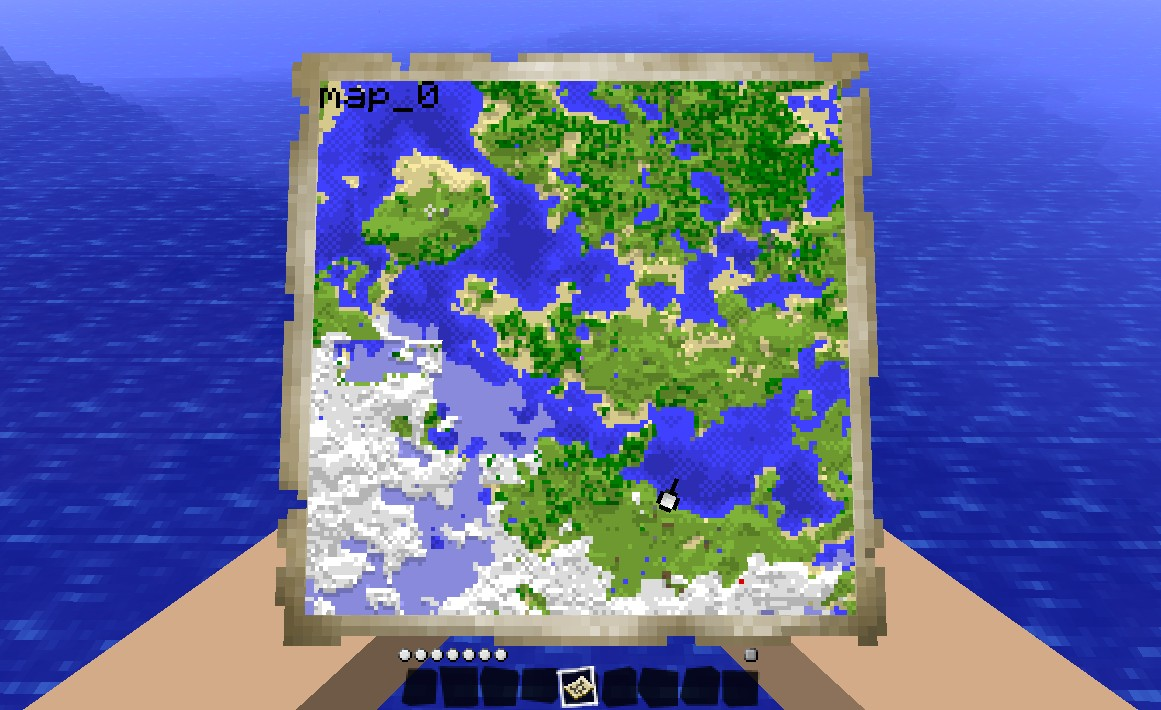
\includegraphics[width=\textwidth]{section01/assets/screenshot_Minecraft.jpg}
\caption[A screenshot of ``Minecraft'']{\label{fig:Screenshot Minecraft}A screenshot of ``Minecraft''}
\end{figure}

\subsubsection{Medieval Fantasy City Generator(MFCG)}
\label{sec:Introduction>Similar Systems>MFCG}
The ``Medieval Fantasy City Generator(MFCG)'' is a web application. This application generates a random medieval city layout of a requested size: small, medium or large, which is made up of different types of regions, and the generation method is stochastic. Furthermore, elements are provided for the user to add to the city, such as farm fields, citadel, plaza, temple, river, coast and so on. Because of the premise of medieval fantasy, the map always includes the walls and castle, but the user can decide whether to display them. It allows the user to edit the map to modify unsatisfying layers using a warping tool. The author also mentioned that the goal of the application is to produce a nice looking map, not an accurate model of a city. Finally, the user can save the map as an image in the ``png'' or ``svg'' format by using the export feature. Figure \ref{fig:Screenshot MFCG} is a screenshot of MFCG.

\begin{figure}[!htb]
\centering
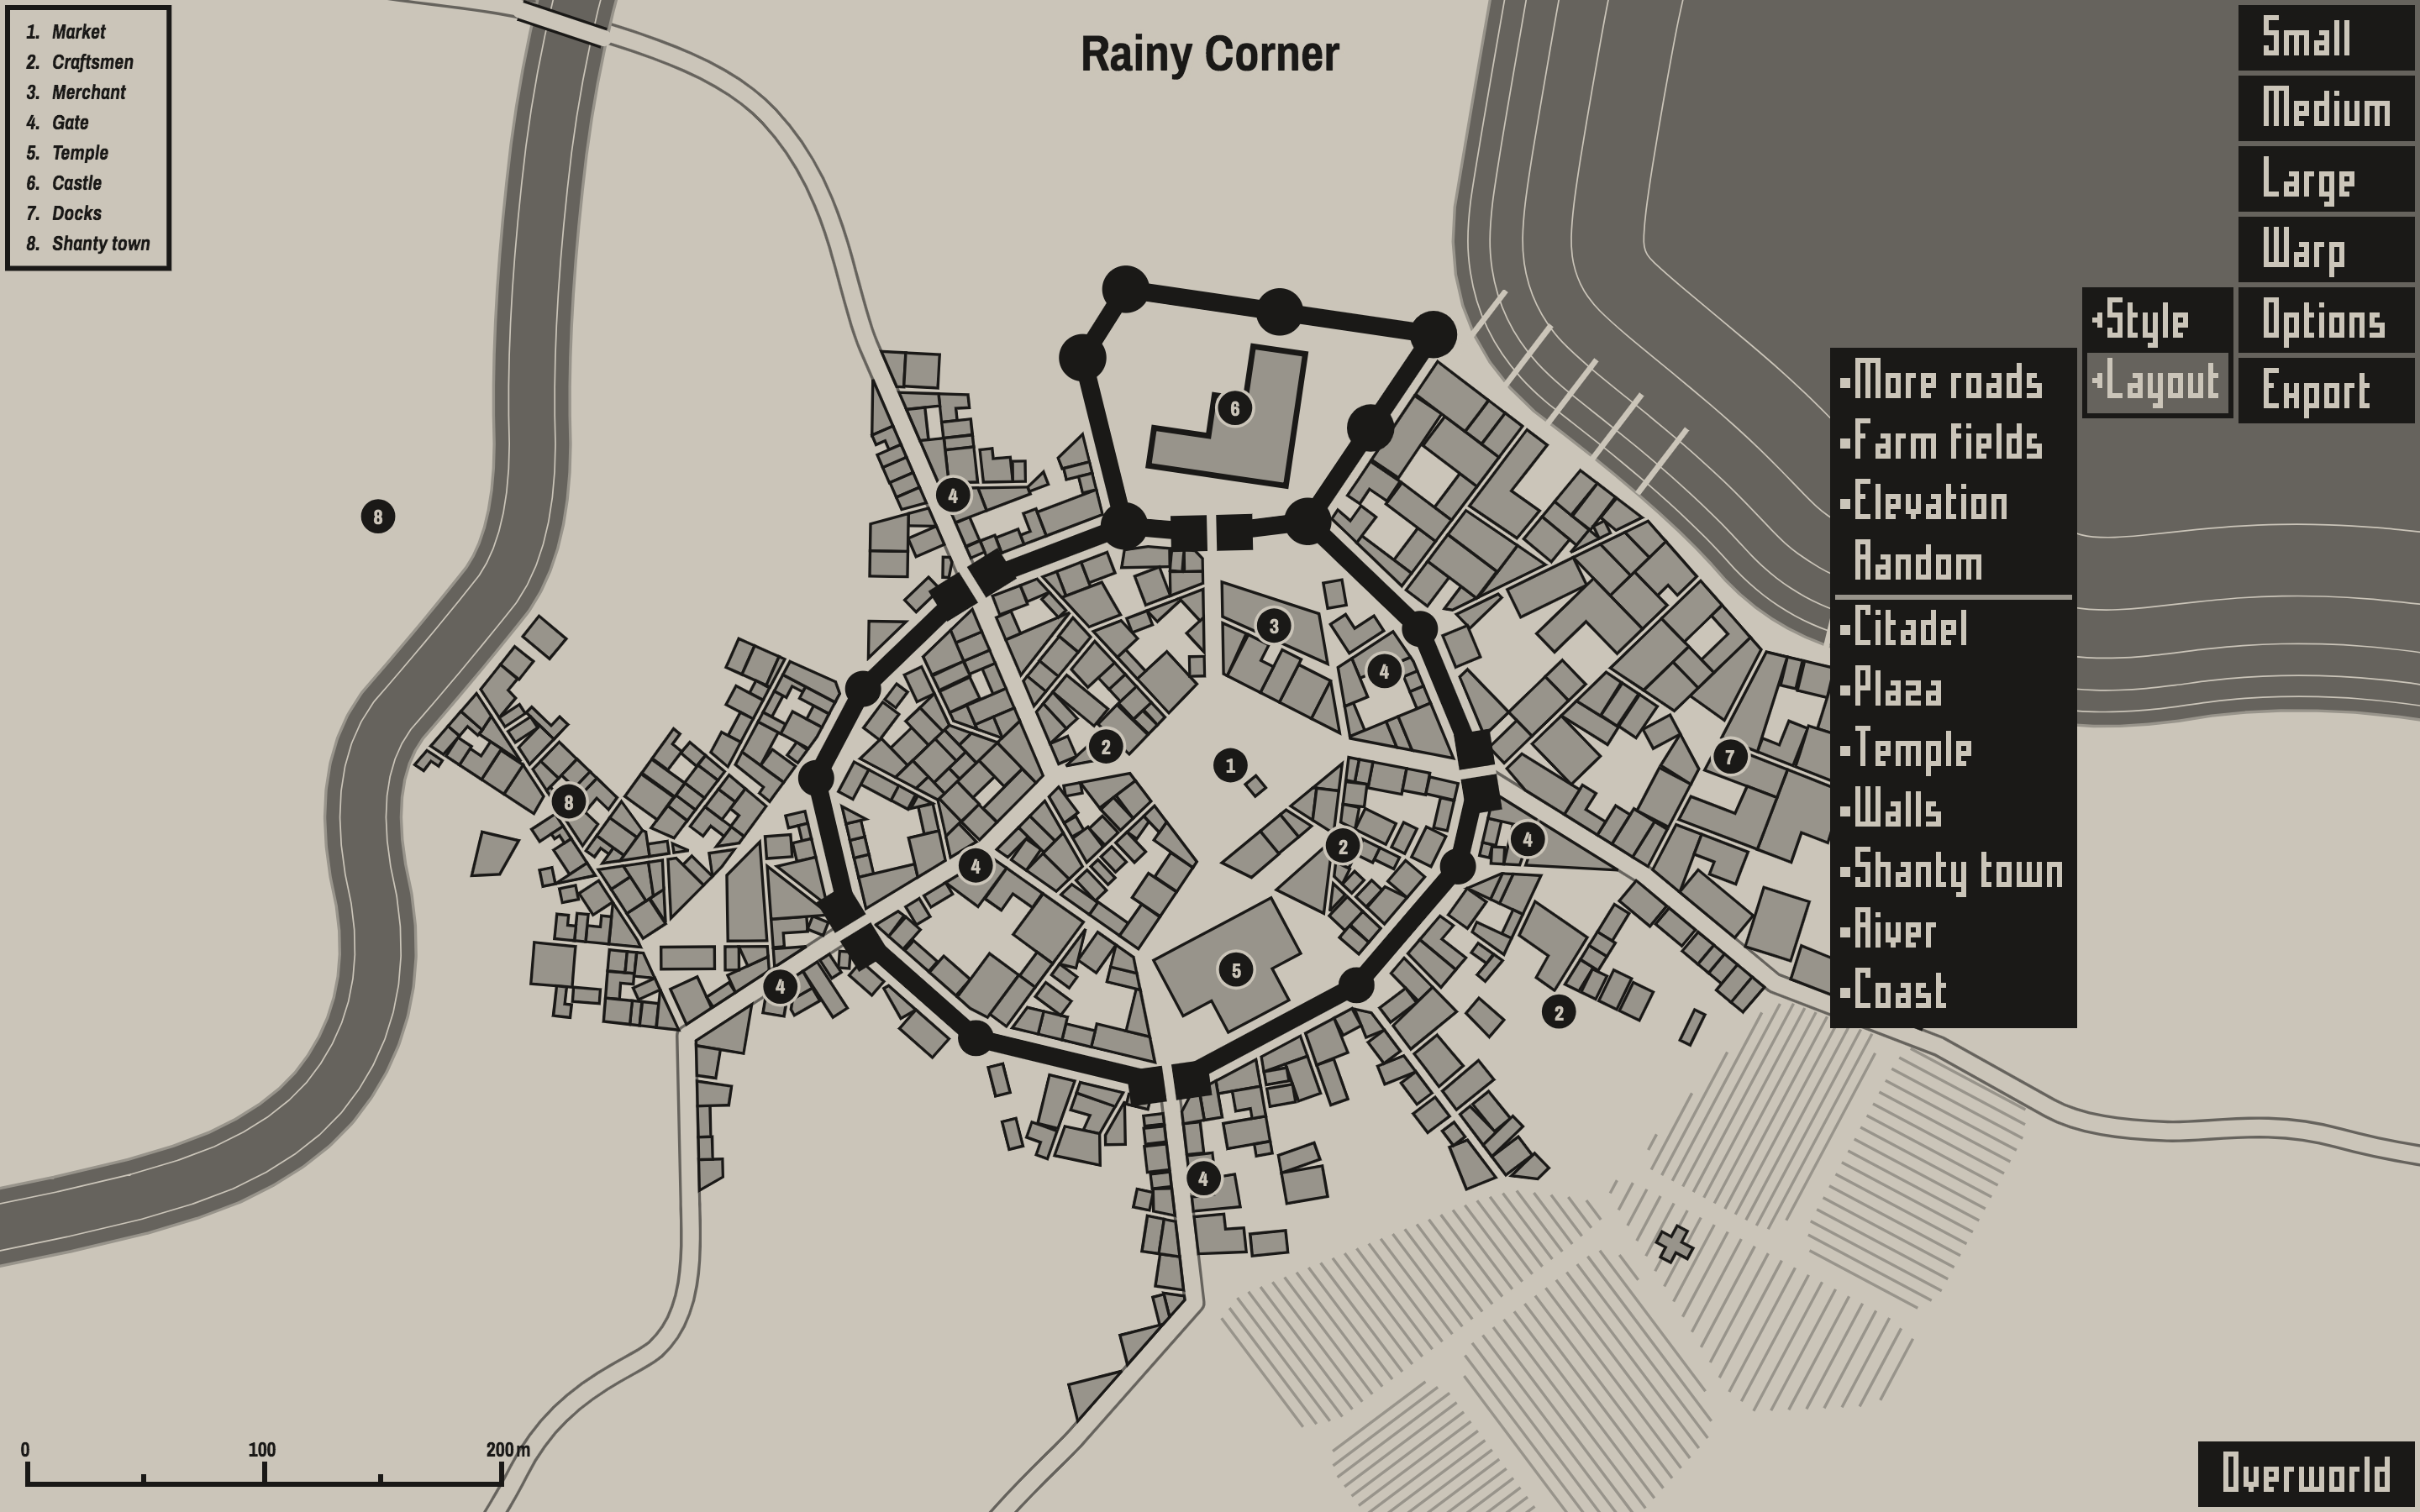
\includegraphics[width=\textwidth]{section01/assets/screenshot_MFCG.png}
\caption[A screenshot of the Medieval Fantasy City Generator]{\label{fig:Screenshot MFCG}A screenshot of the Medieval Fantasy City Generator}
\end{figure}

\subsubsection{Azgaar's Fantasy Map Generator(FMG)}
\label{sec:Introduction>Similar Systems>FMG}
The ``Azgaar's Fantasy Map Generator(FMG)'' is another similar system, which is a larger scale world map. The size of the map made by FMG is not just an island, but a random fantasy map represents a pseudo-medieval world. Just like the real world, the map generated by FMG has constraints that the continent is always surrounded by the ocean and will never touch the border of the map. Although it is a randomly generated map, it is still based on real-world rules. While its most prominent feature is that the user can choose the type of map he likes, which provides the following 5 map types: political, cultural, height, biomes and pure landmass. It also supports user-defined map type, and the user can add additional layers on existing map layers: rivers, temperature, and population. Also, it allows the user to annotate and edit the map using various such editors: layout, style, template, scale, countries, or cultural. It also supports exporting the map in the PNG or SVG format, but unlike the previous application, if the user wants to come back to edit the map in the future, he can save it in the ``map'' format. Figure \ref{fig:Screenshot FMG} is a screenshot of FMG.

\begin{figure}[!htb]
\centering
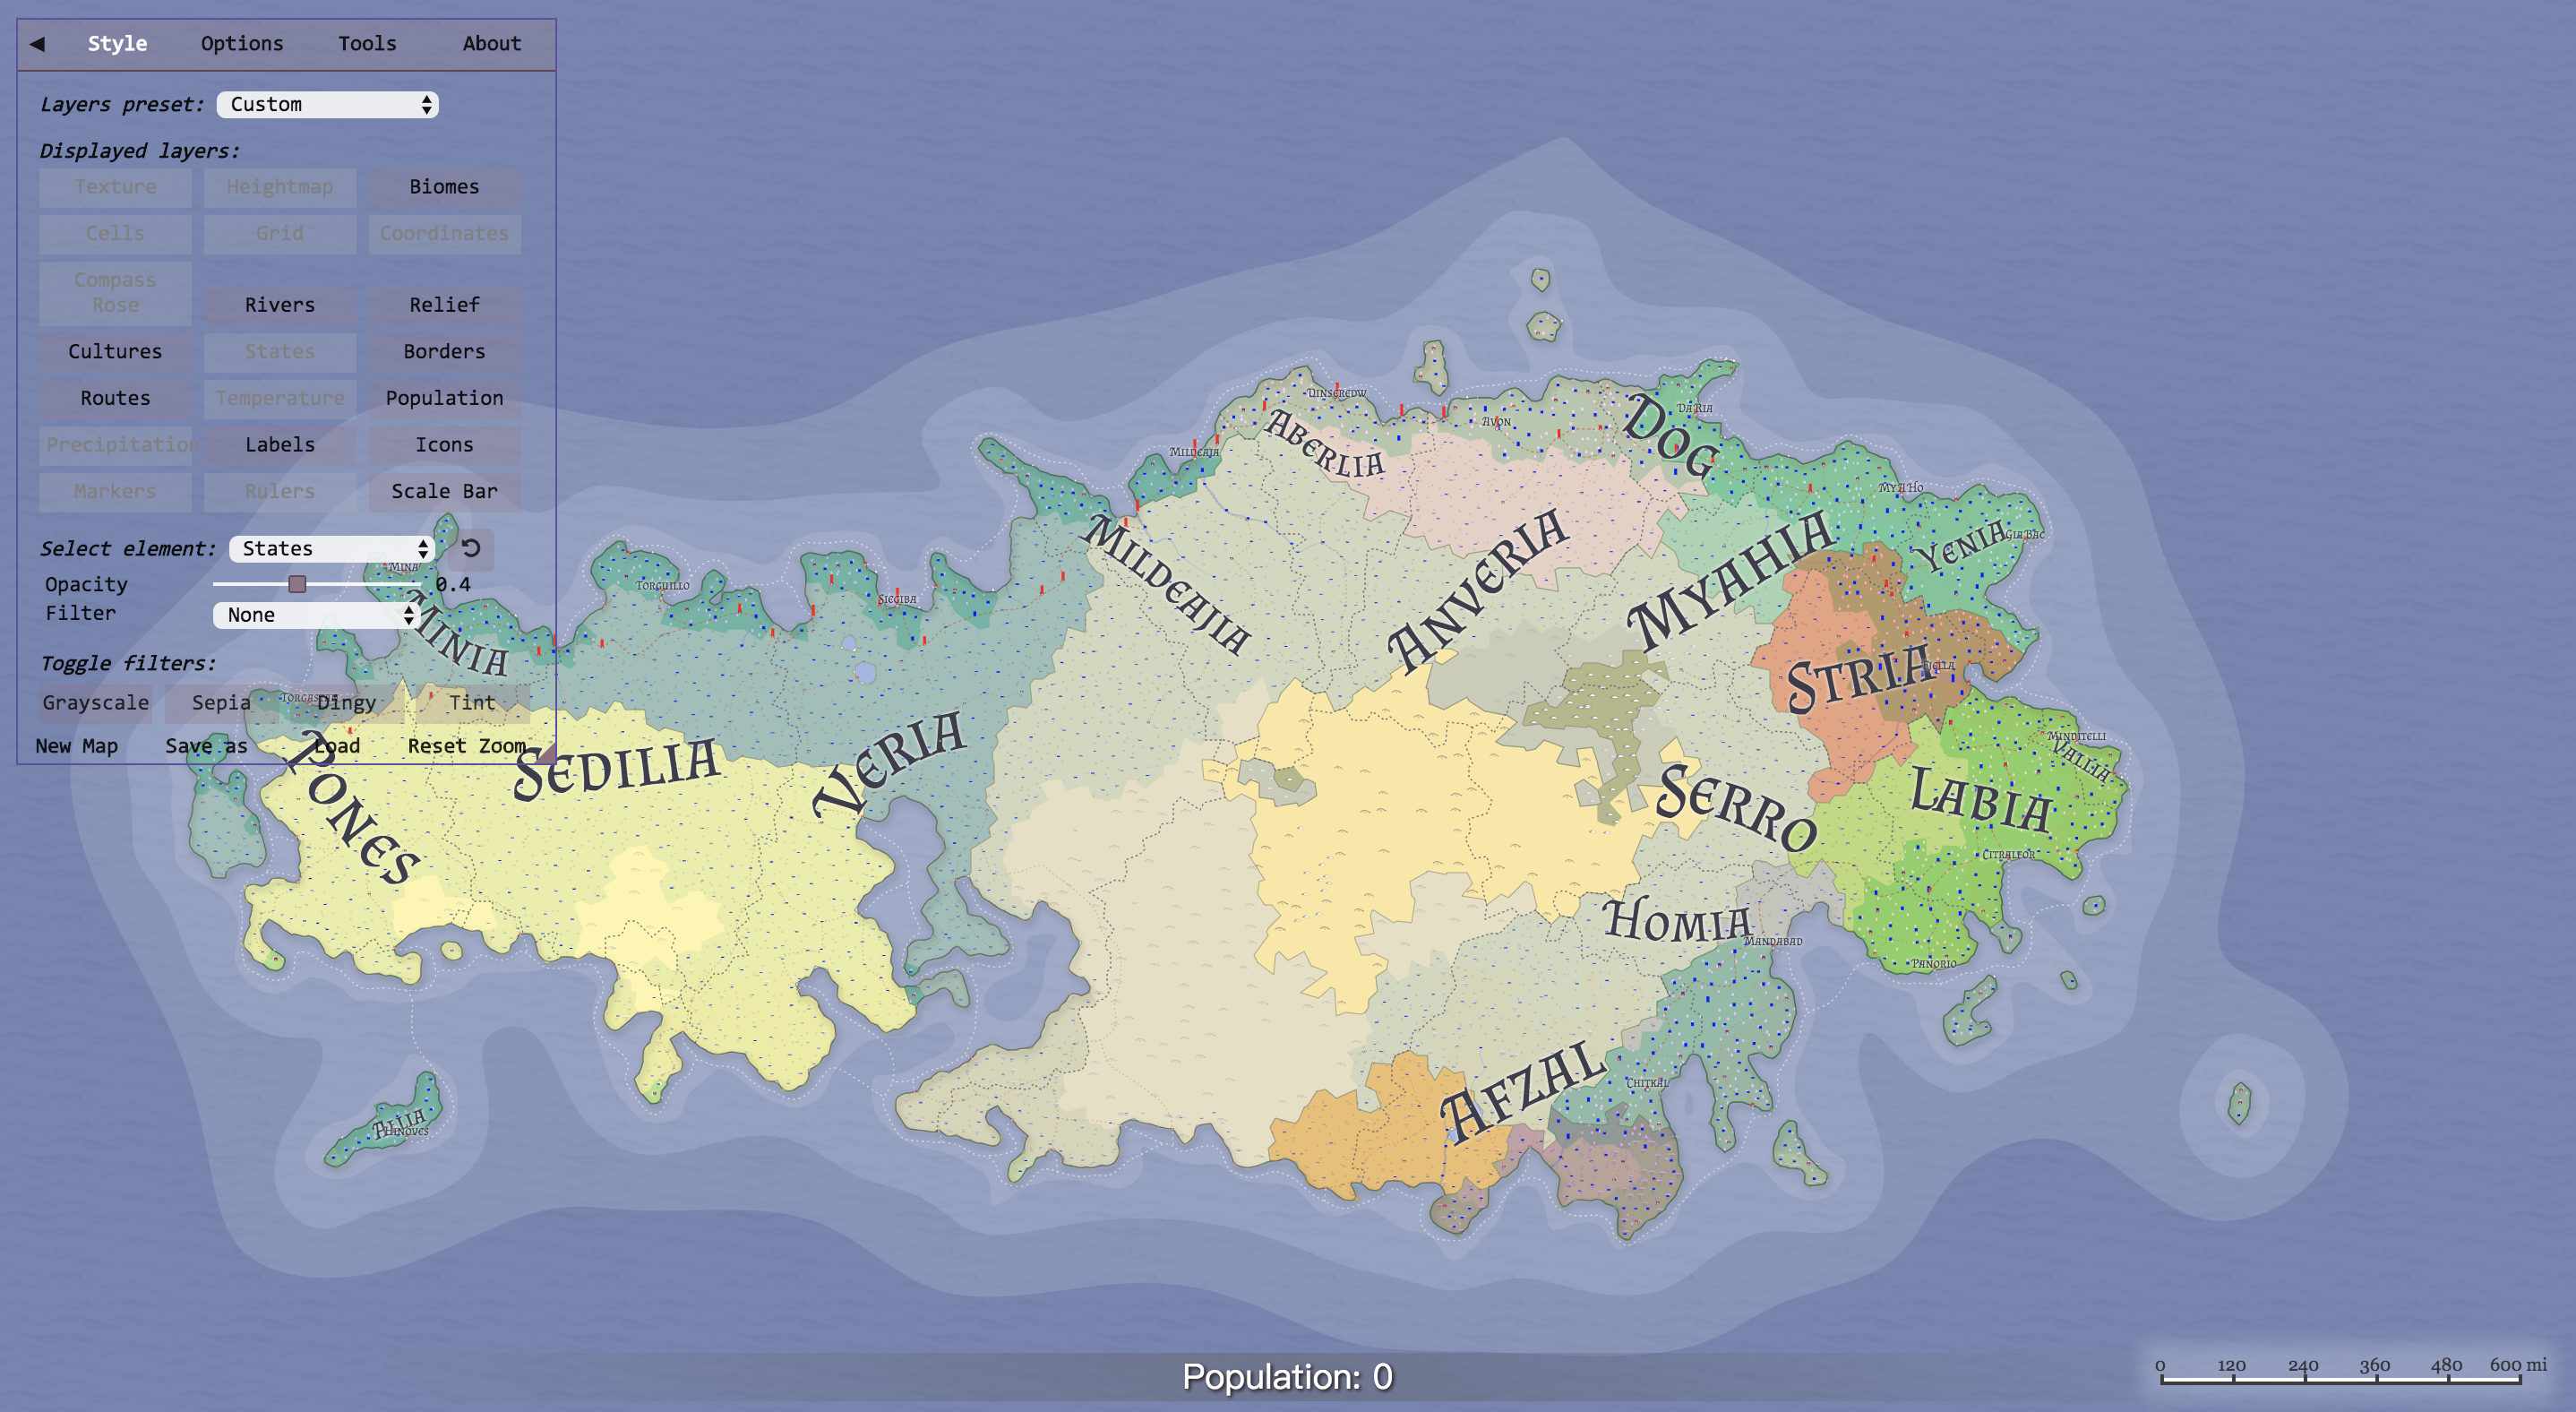
\includegraphics[width=\textwidth]{section01/assets/screenshot_FMG.png}
\caption[A screenshot of the Azgaar's Fantasy Map Generator]{\label{fig:Screenshot FMG}A screenshot of the Azgaar's Fantasy Map Generator}
\end{figure}

\subsection{Project Goal}
\label{sec:Introduction>Project Goal}
The goal of this project is to automatically generate city maps for use in role-playing games (RPG) or worldbuilding narratives. While the ultimate goal of this project is to procedurally replicate maps of a quality similar to the best cartographic hand-created maps by expert artists, we have obtained a modest approximation to the desired level of quality. Our system will have essential features, such as allowing the user to annotate or edit, allowing the user to export the map as an image in the PNG or SVG format, and allowing the user to save it to a database and retrieve it. Figure \ref{fig:Screenshot Metropolist} is a screenshot of the final project.

\begin{figure}[!htb]
\centering
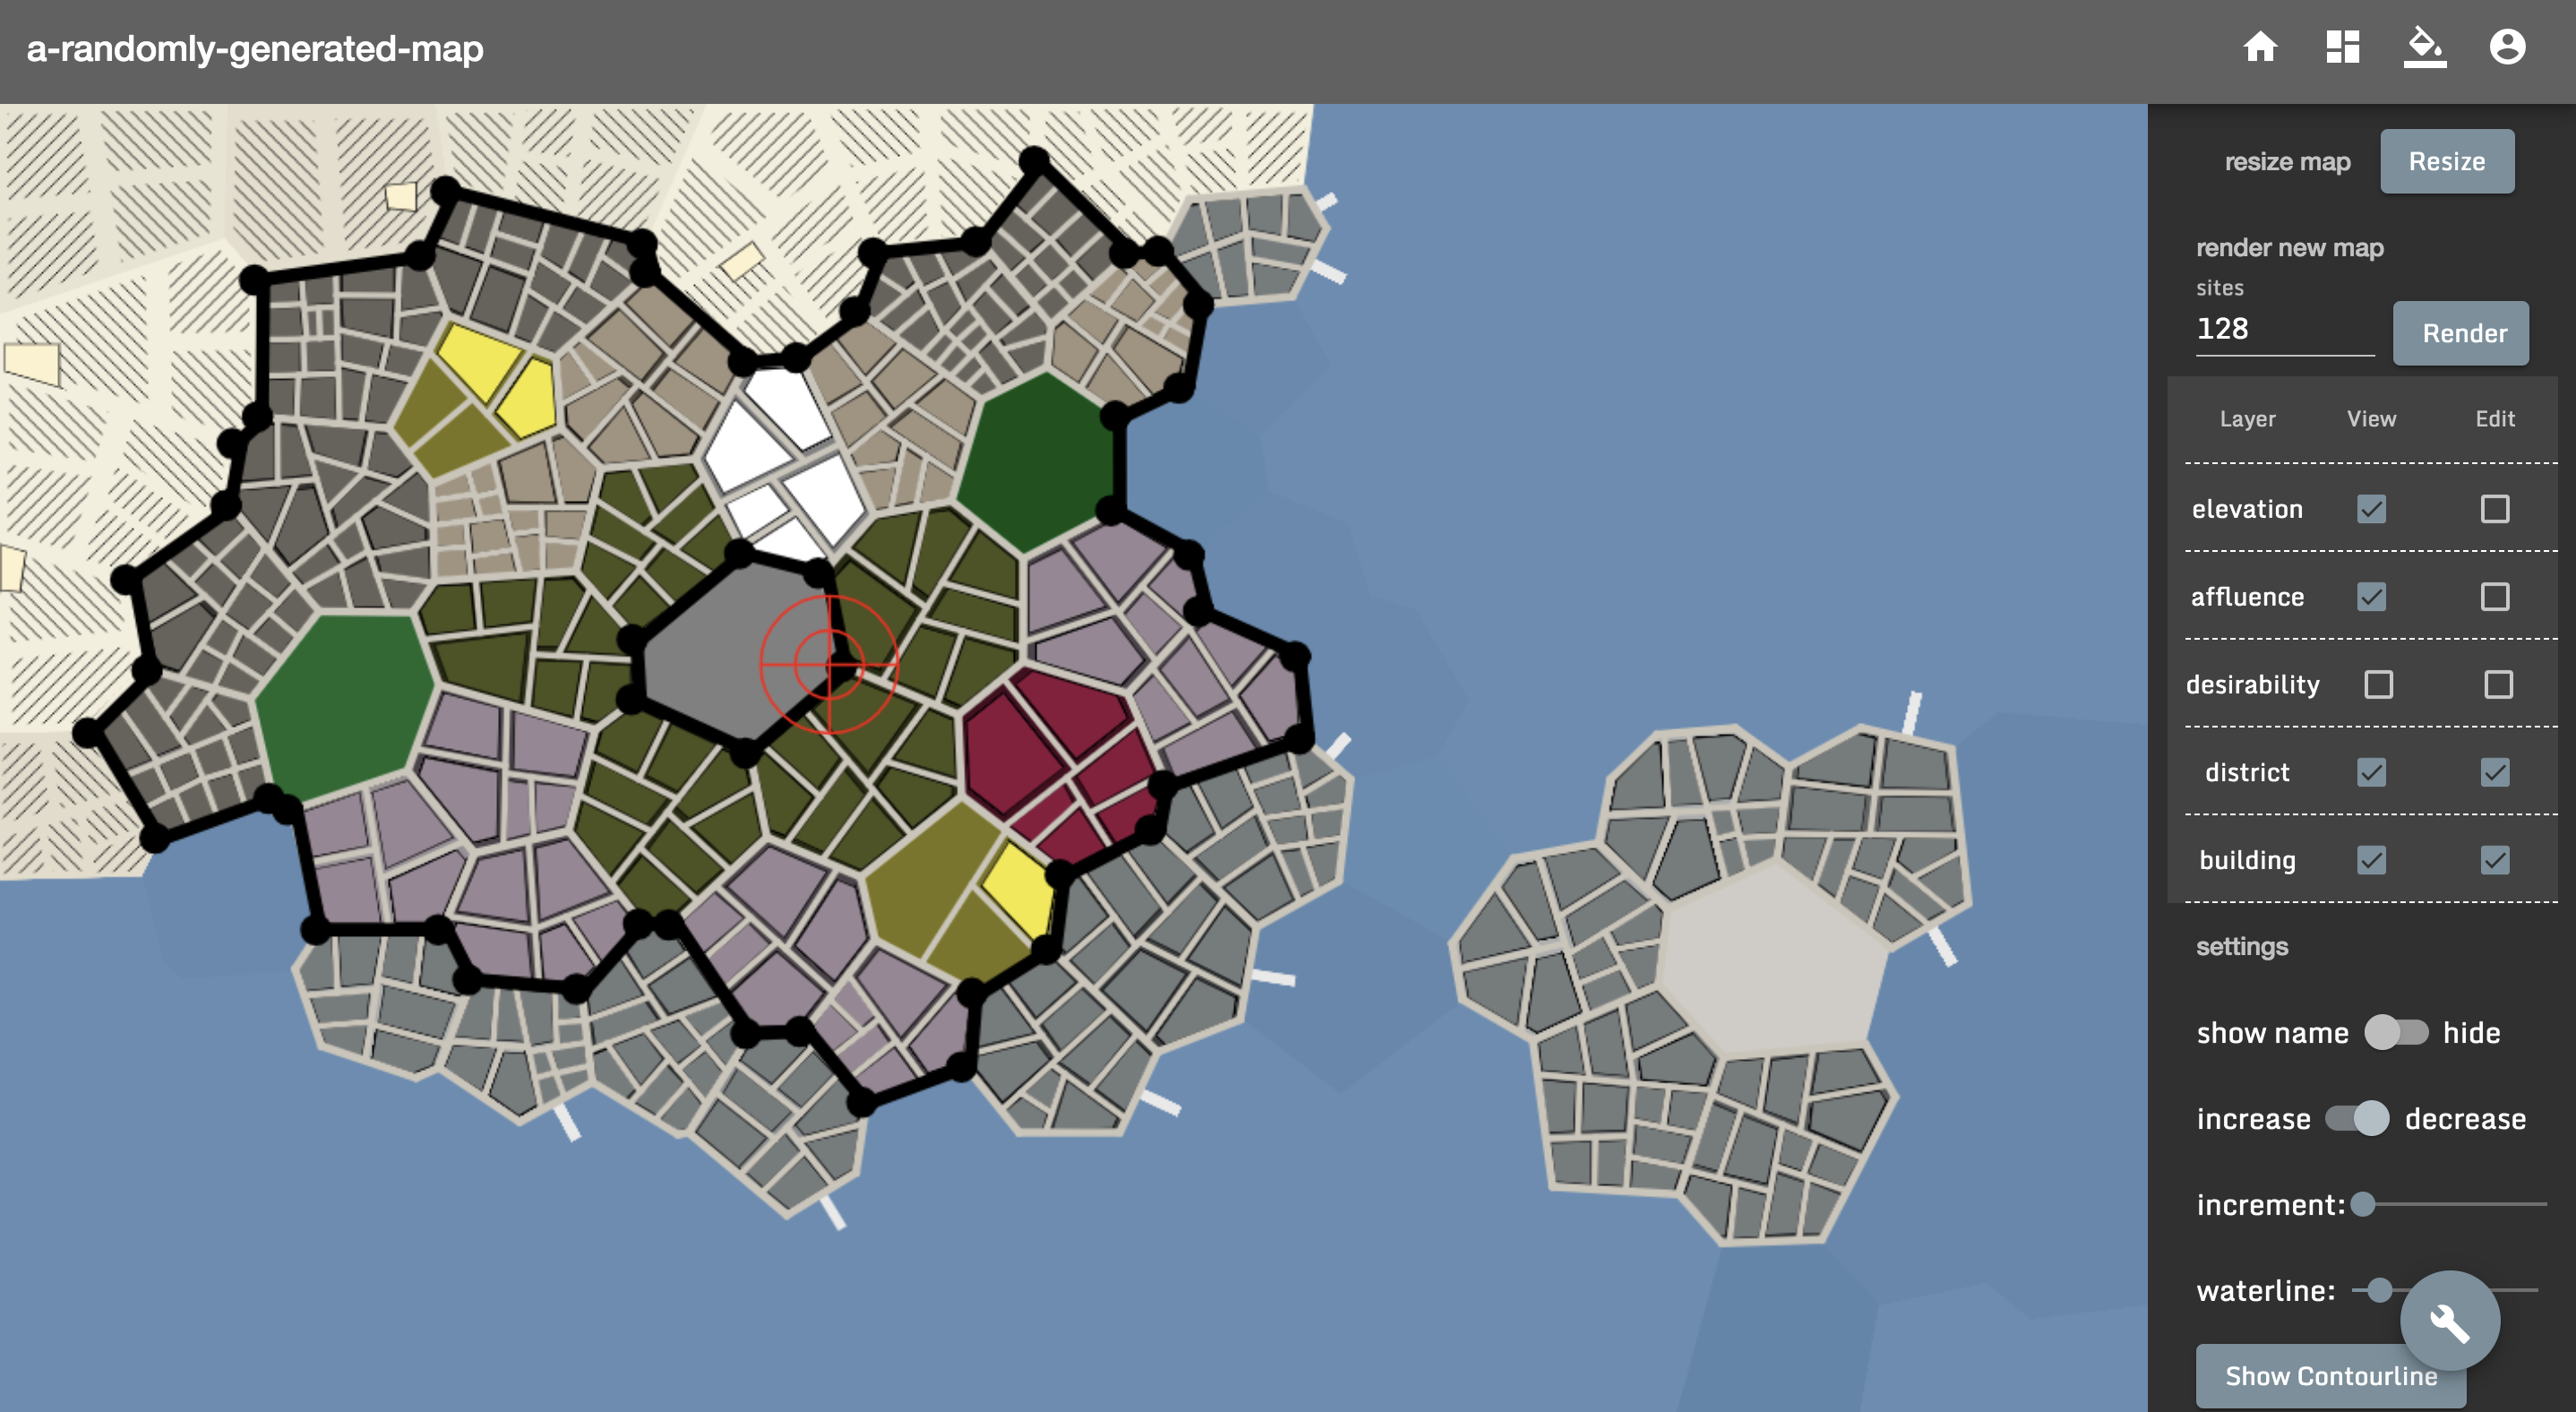
\includegraphics[width=\textwidth]{section01/assets/screenshot_Metropolist.png}
\caption[A screenshot of the current project]{\label{fig:Screenshot Metropolist}A screenshot of the current project}
\end{figure}
